\chapter{Data Collection} \label{chap:data}

As described in Section \ref{sec:ageDB} there are many age-based databases of facial images. However, all existing datasets are based on real age estimation. 

The idea of this work is to compare the performance between predicting real or apparent age labels. In order to do so, a web-based application has been developed using \textit{Facebook's API} to collect a database with these annotations. 

In order to increase the number of images in the database, an exhaustive research was done to find similar applications which were collecting the same, or very close, type data. The result of this search was AgeGuess\footnote{AgeGuess: \url{http://www.ageguess.org/}} a web-based application developed by Dusan Misevic\footnote{Dusan Misevic is a researcher at Max-Planck Odense Center on the Biodemography of Aging, Biology department of the SDU} and 
Ulrich Steiner\footnote{Ulrich Steiner is a researcher at the Center for Research and Interdisciplinarity in Paris, of the INSERM Unit 1001}, which collects nearly the same information as the collected for this work. The line of research of the AgeGuess team is focused on ageing and age perception from a biologically demographical point of view. The AgeGuess team agreed to partner with the HuPBA research group and the ChaLeran platform to joint effort in the data collection.

\section{Web Application}

The aim of the web-based application was to speed up the collection and labelling processes and reach more people with broader backgrounds to create an age database as diverse as possible. These processes were implemented in a gamified \footnote{Gamification is the use of game thinking and game mechanics in non-game contexts to engage users in solving problems and increase users' self contributions \cite{Deterding:2011:GDE:2181037.2181040}.} fashion so the experience of the users with the application was satisfactory and engaging. 

The application uses the API of Facebook to create a ranking with the user's Facebook friends and adding a factor of competitiveness to the game. It is also used to collect information about the labellers such as gender, age and nationality.

\begin{figure}[!h]
	\centering
	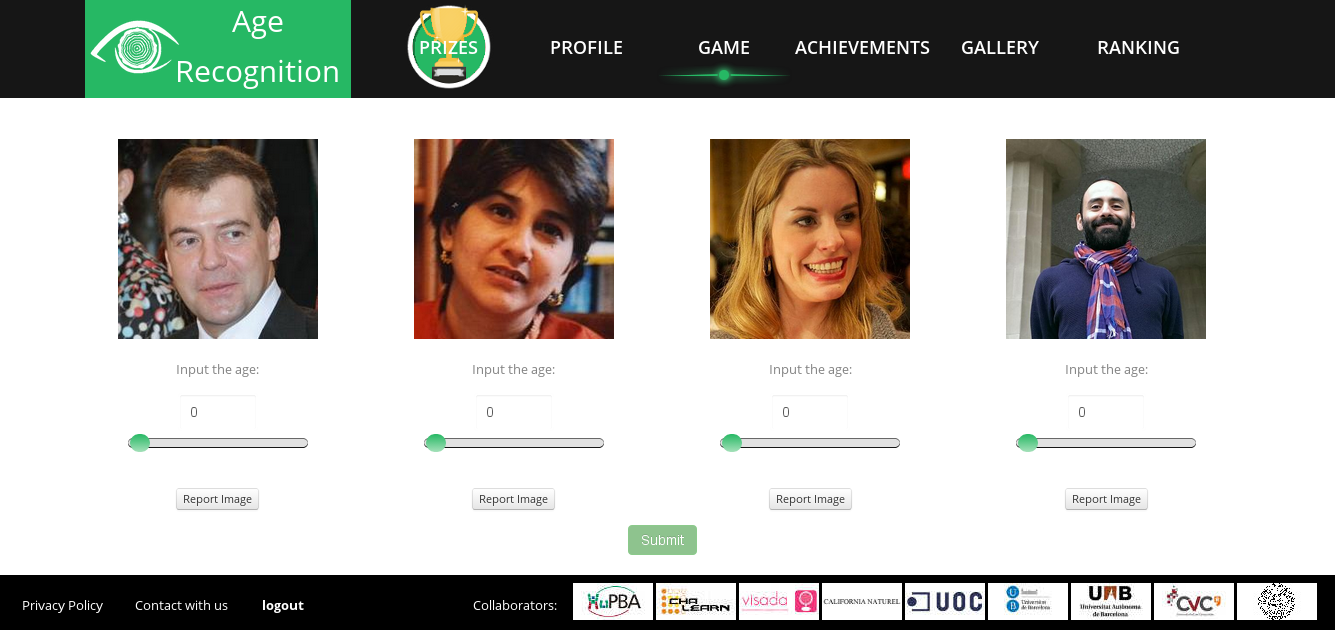
\includegraphics[width=\textwidth]{figures/age_app_1}
	\caption{Age Recognition Application: Game Panel}
	\label{fig:game}
\end{figure}

\begin{figure}[!h]
	\centering
	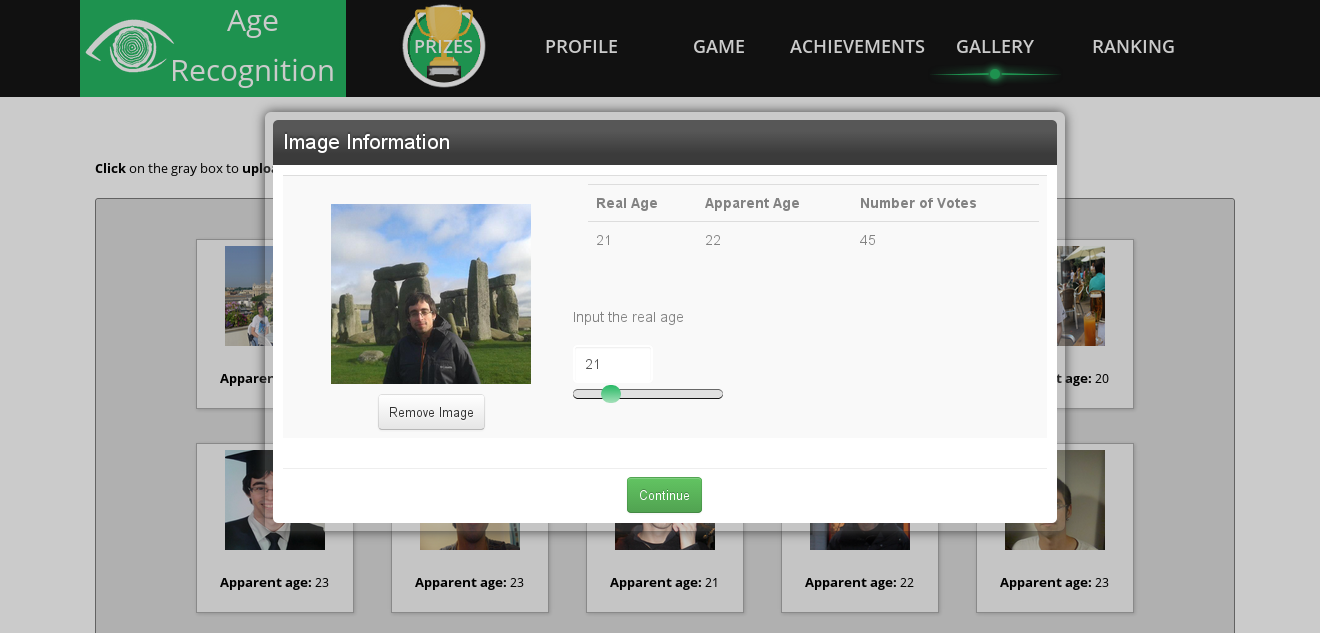
\includegraphics[width=\textwidth]{figures/age_app_2}
	\caption{Age Recognition Application: Gallery Panel}
	\label{fig:gallery}
\end{figure}

\begin{figure}[!h]
	\centering
	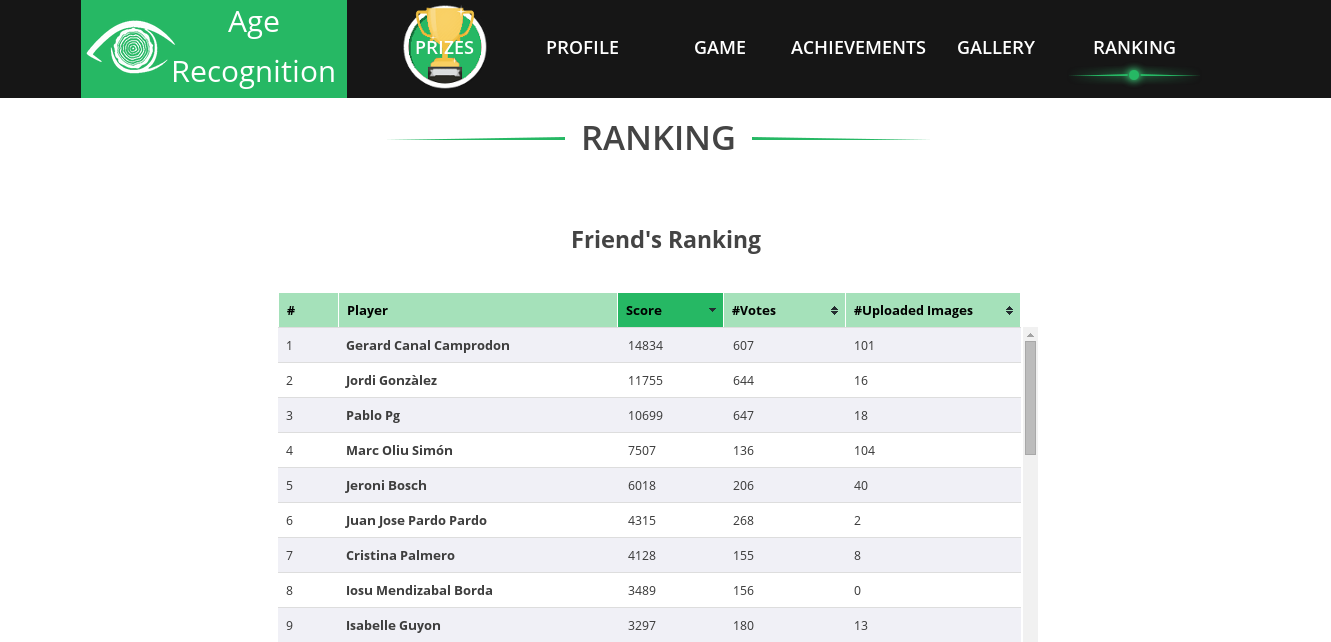
\includegraphics[width=\textwidth]{figures/age_app_3}
	\caption{Age Recognition Application: Ranking Panel}
	\label{fig:ranking}
\end{figure}

\subsection{Gamification Strategy}
The web-application is basically a platform to label and upload images, which is not funny or motivating. However, using gamification techniques the labeller engagement can be increased. The gamification strategies used were mainly four:

\begin{itemize}
	\item The users or players get \textbf{points} for uploading and voting (labelling) images. The closer the vote is to the apparent age (average current voted age) the more points the player gets. This strategy is pretended to persuade the users to wrongly label the images.
	\item Two \textbf{ranking} tables are shown to the users, one with the ranking positions of the users' Facebook friends and another showing the global classification. This strategy was created with the purpose of increase engagement between users, making them compete with each other. 
	\item A system of \textbf{achievements} was implemented, including the four types of achievements shown in the Table \ref{tab:achiev}.
	\begin{table}[!h]
		\centering
		\begin{tabular}{l|l}
			\textbf{Achievement} & \textbf{Description} \\ \hline
			Share it! &	Invite your friends to play and you will get stars.	\\
			Precision &	The better your guesses, the higher your rank. \\
			Vote! &	Vote on more images to get more stars.\\	
			Add Pictures! &	Upload more images to get more stars. \\
		\end{tabular}
		\caption{List of achievements with its description}
		\label{tab:achiev}
	\end{table}
	\item Thanks to one of the Challenge sponsors, California Naturel \footnote{\url{http://www.californianaturel.com/}}, a bunch of cosmetic lots were offered as a \textbf{prize} for the ones who led the global ranking. The aim of the prize was to push participation further.
\end{itemize}


\subsection{Application Structure}
When users access the web for the first time they have to register using their Facebook account and accept the terms and conditions for the application usage (further explanation of the legal terms in the Appendix \ref{cha:TaC}). After registration the \textit{How to play} panel will be displayed giving a short description of all the parts of the application.

As it is shown in Figures \ref{fig:game}, \ref{fig:gallery} and \ref{fig:ranking}, at the top of the site, there is a control menu that allows the users to move through the site with just one click. A description of the different panels is written below:

\begin{itemize}
	\item \textbf{Profile}: In this section the users can keep track of their statistics (Number of uploaded images, number of votes, points obtained and global ranking position).
	\item \textbf{Game}: This is the main section (Figure \ref{fig:game}), four images are shown at the same time and the users are asked to guess the age of all of them. They can report the images if any of them is considered offensive, bad quality, more than one person appears in the image, etc.
	\item \textbf{Achievements}: In this panel users can keep track of their achievements and shows the next goals.
	\item \textbf{Gallery}: In this section (Figure \ref{fig:gallery}) players are able to see the images they have uploaded and see how many people have voted on them and get an estimation of their apparent age according to other users opinion. They are also able to upload new images in this panel, while uploading they are asked to crop (if necessary) and specify the real age of the person in the image.
	\item \textbf{Ranking}:	The last panel (Figure \ref{fig:ranking}) allows users to compare their scores with their Facebook friends in the \textit{Friends Ranking} and to all the players in the \textit{Global Ranking}.
\end{itemize}

\subsection{Troubleshooting}\label{sec:trouble}

When creating a public image database there are at least two things to keep in mind: image quality and image license.

To have good quality images the users are asked to upload images of a single person, preferable a portrait. In order to facilitate these requisites, the option of cropping the image is given in the uploading step. Also a minimum image size is enforced to avoid tiny images to be uploaded.
 
When users first register in the website they are asked to read and accept the terms and conditions which establish that the uploaded images rights must be hold by the user or the images have a license that allows the use of them and their redistribution free of charge. The users are also warned that the images will be used for research purposes and will be publicly available for this use. 


\section{HuPBA-AgeGuess Dataset}

This section will describe and analyse the collected database called HuPBA-AgeGuess Dataset.  

The Table \ref{tab:charact} shows the main characteristics of the database. The web application gathered more than 1500 images and almost 15000 votes, which means almost 10 votes per image in average.

\begin{table}[h]
	\centering
	\begin{tabular}{|c|l|l|l|l|}
		\rowcolor[HTML]{EFEFEF} 
		\hline
		\multicolumn{2}{|l|}{\cellcolor[HTML]{EFEFEF}\textbf{Features}} & HuPBA & AgeGuess & Total \\ \hline
		\multicolumn{2}{|l|}{Images}                                    & 1506  & 33592 & 4865\\ \hline
		& female                & 44  & 1828 & 1872  \\ \cline{2-3} 
		\multirow{-2}{*}{Users}                 & male                  & 110 & 1143 & 1253 \\ \hline
		& female                & 1753  & 75136 & 76889\\ \cline{2-3} 
		\multirow{-2}{*}{Votes}                 & male                  & 14897 & 53117 & 68004\\ \hline
	\end{tabular}
	\caption{HuPBA-AgeGuess Database Characteristics}
	\label{tab:charact}
\end{table}
	
The ages distribution of the database (Figure \ref{fig:distr}) is not uniform as ideally should be, but instead contains more instances of people with ages between 20 and 30 than the rest of ages. There is also a very low incidence of individuals under 15 years old and over 70 years old. It can also be observed that both real and apparent age have a very similar distribution. This age distribution is justified by the fact that the people that most use social media are in between 18 and 49 years old \cite{brenner201372}.

\begin{figure}[h!]
	\centering
	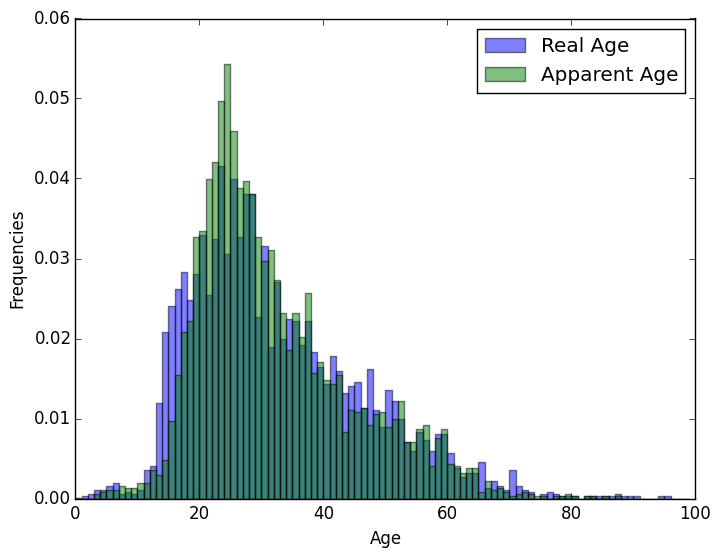
\includegraphics[width=\textwidth]{figures/Label_Distribution}
	\caption{Labels Distribution}
	\label{fig:distr}
\end{figure}

Figure \ref{fig:apparent_real} shows the apparent age of all the images sorted by real age. The apparent age is fitted into a curve that shows how younger people (0 - 25 years old) is overestimated while older people (50 - 100) is under estimated. The Figure \ref{fig:apparent_real} also shows that the ages where the apparent age has more variance are in between 18 and 30 years old.

\begin{figure}[h!]
	\centering
	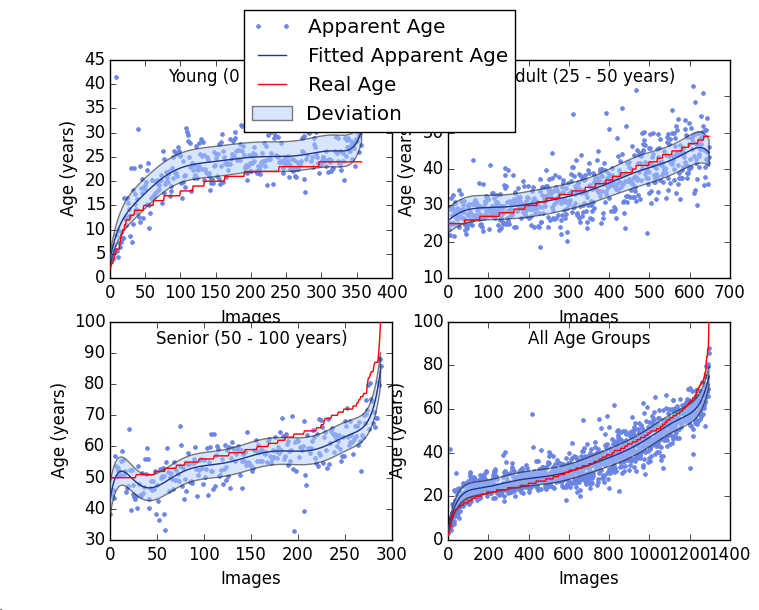
\includegraphics[width=\textwidth]{figures/Labels_across_img}
	\caption{Apparent age }
	\label{fig:apparent_real}
\end{figure}

In Figure \ref{fig:gender} illustrates a comparison between Male and Female age perception, which lids to think that the differences is not significant (if any).

\begin{figure}[h!]
	\centering
	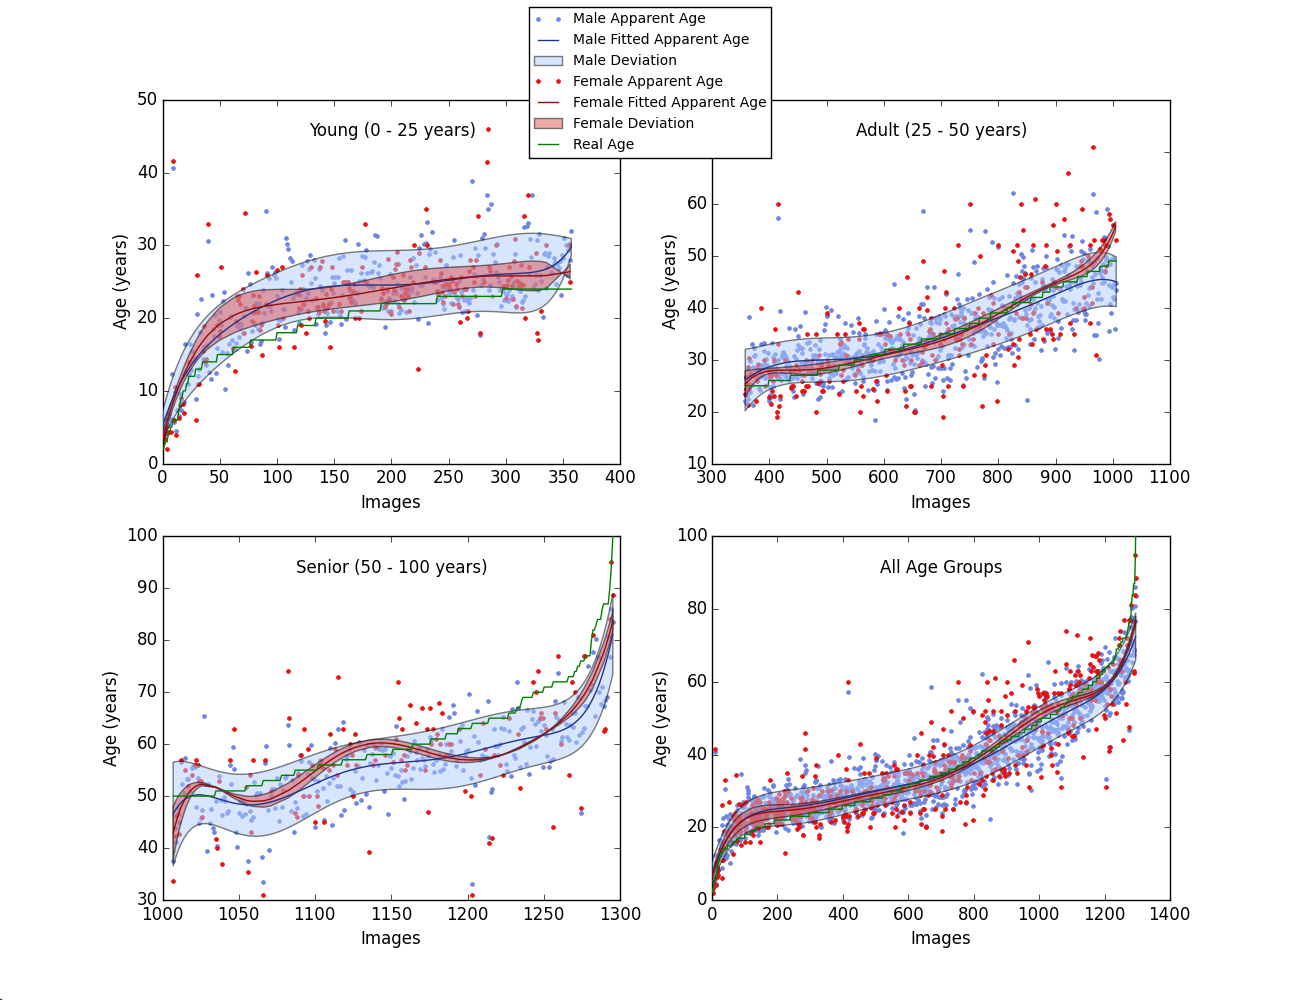
\includegraphics[width=\textwidth]{figures/Labels_across_img_gender}
	\caption{Comparison between Male and Female age perception.}
	\label{fig:gender}
\end{figure}

\begin{figure}[h!]
	\centering
	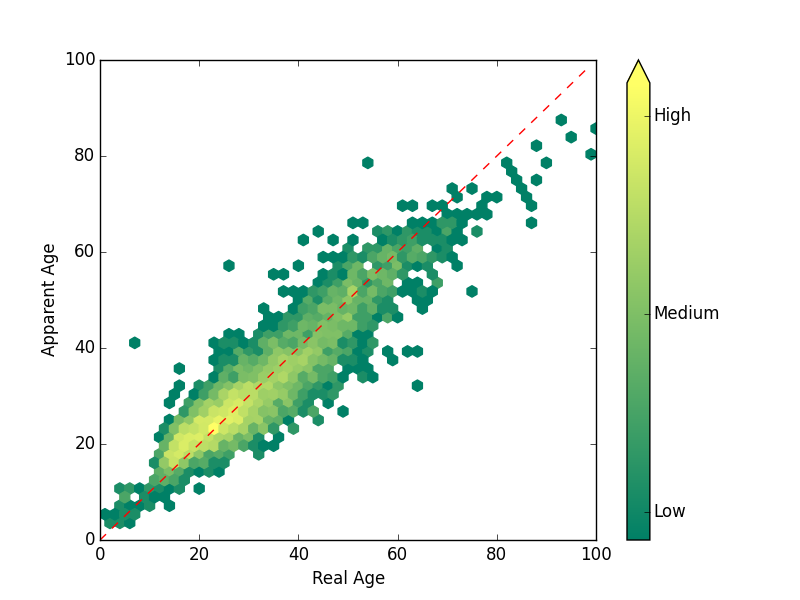
\includegraphics[width=\textwidth]{figures/real_vs_apparent_summer}
	\caption{Real vs. Apparent age.}
	\label{fig:RvsA}
\end{figure}

As a summary, some of the properties of the database are listed below:

\begin{itemize}
	\item Thousands of faces labelled by many users.
	\item Images with background.
	\item Non-controlled environments.
	\item Non-labelled faces neither landmarks, making the estimation problem even harder.
	\item The first datasets in the literature including
	estimated age labelled by many users to define the ground truth with the objective of estimating the age.
	\item The dataset also provides for each image the real age, although it is not used for recognition (just for analysis purposes).
\end{itemize}
